\documentclass[journal]{IEEEtran}
\usepackage{amsmath,amsfonts}
\usepackage{algorithmic}
\usepackage{algorithm}
\usepackage{array}
\usepackage[caption=false,font=normalsize,labelfont=sf,textfont=sf]{subfig}
\usepackage{textcomp}
\usepackage{stfloats}
\usepackage{url}
\usepackage{verbatim}
\usepackage{graphicx}
\usepackage{cite}
\usepackage{xcolor}
\usepackage{parskip}
\usepackage{amsthm}
\usepackage{soul}
\usepackage{hyperref}
\usepackage{listings}
\usepackage{tabularx}
\lstset{
  basicstyle=\ttfamily,
  columns=fullflexible,
  breaklines=true,
  postbreak=\mbox{\textcolor{red}{$\hookrightarrow$}\space},
}
\hyphenation{op-tical net-works semi-conduc-tor IEEE-Xplore}
% updated with editorial comments 8/9/2021

\begin{document}

\title{An Investigation into the Effectiveness and Impact of a Continuous Delivery Pipeline upon University-Level Game Development Teams}

\author{Frost Donovan (REPLACE WITH STUDENT NUMBER FOR SUBMISSION)}

\maketitle

\begin{abstract}
    % What's the problem? What am I looking at? How does that help solve the problem? 
    % Opening, Challenge, Action, Resolution 
    REPLACE WITH OCAR FORMAT. OPEN WITH CHALLENGE CONTEXT (STAKEHOLDER CONFIDENCE \& SCOPE CREEP). POISE CD AS A SOLUTION TO THIS CHALLENGE, A SOLUTIONS TEAM'S HAVE NOT HISTORICALLY USED. DISCUSS IMPLEMENTATION OF PIPELINE. TALK BRIEFLY ON OTHER CD BENEFITS
    Continuous Delivery (CD) is a technique designed to increase reliability and consistency with delivery of builds. This can then help to increase frequency of testing, the accountability of the development team, as well as the teams transparency and shared understanding of the projects state. This can increase team moral as well as stakeholder confidence, as both are able to regularly see the current state and rate of progress for the project. This encourages regular analysis of development pace and project scope, both internal and external. This stakeholder confidence and awareness of scope is a common problem within student development teams, so this investigation will answer to what extent the deployment of a CD pipeline will help to reduce these problems.
\end{abstract}

\section{Introduction}
EXPAND UPON CHALLENGE FACED. INCLUDE ROADMAP AT END OF INTRO (ROADMAP OF WHAT?). FRAME THROUGH LENS OF SOLVING A PROBLEM. ARTICULATE WHY IT IS WORTH SPENDING TIME AND RESOURCES CONUCTIONG THE INVESTIGATION - JUSTIFY BENEFITS OUTWEIGHING THE COST OF RESEARCH
The intention of this paper is to act as an initial investigation into the effects of a Continuous Delivery (CD) pipeline on student development team's. Student team's often have a problem with project scope and reliability of delivering regular builds, which the reported benefits of CD should help with. As such, this study will consist of a case study of a number of student team's within Falmouth University Games Academy across the entire department, with half the participating team's being provided with a CD pipeline and data being gathered throughout the study by survey. Through this study we will seek to provide some initial answers to whether a CD pipeline can positively effect developer \& project supervisor confidence, understanding of the project's state, and project scope.

\section{An analysis of Continuous Delivery}
\subsection{What is Continuous Delivery?}
Continuous Delivery (CD) is an expansion of Continuous Integration (CI), a pipeline for the continuous integration of code, being developed on separate branches, into the main branch. This code is merged into the main branch and then tested to ensure there are no merge conflicts or obvious errors thrown from the combined code. Assuming all of these tests pass, this merged code is pushed to the project repository. A key part of this pipeline is that the entire process is automated, ensuring minimal time is wasted waiting for tests to run or code to be uploaded.\cite{ContDelIntro,CICDCD} \\
CD takes this one step further, in that after a project passes through the CI pipeline, the code is then compiled, packaged, and further tests that require the project to be compiled can be run. These tests should not be run before other tests that don't require compilation due to Fail Fast principles\cite{shore2004fail,bamboo}. Assuming there are no failures during compilation or testing, the built program can then be uploaded to somewhere where it can be easily accessed. Here, it is important to make a distinction between Continuous Delivery, where the build is available internally but not to users, and Continuous Deployment, where the build is pushed straight out to the current product users. This practice is core to the agile methodology, in fact being the first point on the agile manifesto\cite{agilemanifesto}.

\subsection{Benefits \& Drawbacks of CD}
The primary benefit of CD is reduced cycle time - a reduction in the time it takes for a change in the project to happen and then for the user to have that change applied to their version of the software. This principle is core to the agile methodology, being the very first principle in the agile manifesto\cite{agilemanifesto}. This faster cycle time means that feedback from active users can be obtained much quicker, both on the effectiveness of bug fixes and also on new features. Agile is designed to avoid the pitfalls of Waterfall\cite{royce1987managing}, one of which is the commitment of significant time and/ or resources into features that either are unattainable, or not actually wanted by the user. While other agile methods, such as Scrum or Extreme Programming\cite{cohen2004introduction,agilewithscrum}, can be an important part of the agile process, the effectiveness of a development team in delivering \textit{value} is always going to be dependant on the speed and reliability with which user feedback can be obtained. \\
A benefit of this fast cycle time is that not only are players able to see these changes faster, but stakeholders and publishers are able to see development progress, both regularly and on demand. This can be a significant step to building trust between a development studio and publisher, especially if the studio is new or doesn't have an existing relationship with the publisher\cite{gamedevhandbook}.

Part of the CD pipeline is testing, with a suite of unit tests being run on the code as part of the build process. As this build process is run consistently, rather than all at once leading up to a main release, this means bugs are found incrementally, stopping the accumulation of technical debt, reducing the cost to fix bugs, and reducing stress on programmers by preventing an overwhelming influx of bugs. While these unit tests will likely catch a lot of bugs, some bugs will only be caught during human playtesting. This decreased cycle time means that human playtesting can happen sooner \& more regularly, and fixes are delivered to testers \& players almost immediately, rather than having to wait for the next release window.

Another strength of a Continuous Delivery pipeline is that it is fully automated. This allows less developer time to be spent setting up build or test environments and manually going through the build process, and more time on actually creating the product. This can be a \textit{significant} time save, with some large scale projects reportedly taking weeks to set up environments ready to produce a release build\cite{paddy, ContDelIntro}. This system also significantly reduces the chance that there are any errors caused by mistakes during the build process as this build-release pipeline will have had many iterations of the product pass through it, before a major release deadline. This increases the reliability and stability of new releases.

\section{Case Studies \& Supporting Literature}
With these benefits in mind it raises two questions; \\
If a CD pipeline is this important and valuable, is it being taught to new developers in further education?, and \\
If it is, is it actually as effective in practice with student teams as it is in theory?

There is limited literature relating to Continuous Delivery being implemented in an academic context, and \textit{no} literature that I could find of this being implemented in a game development context. Even upon reviewing a literature review on rapid releases\cite{mantyla2015rapid} there were \textit{no} references to this within a games development context. This lack of literature provides a problem when attempting to find evidence on the performance of CD pipelines, however does highlight a \textit{need} for further literature and case studies on the subject. There is even a lack of literature relating to the effectiveness of CD pipelines within an industry setting.

Relating to the effect of CD pipeline deployment in an industry setting, the literature review mentioned above by M{\"a}ntyl{\"a} et al.\cite{mantyla2015rapid} carried out an investigation into firefox's transition "from a TR [Traditional Release] model of one release a year to an RR [Rapid Release] model where new releases come every 6 weeks" \cite[p.2]{mantyla2015rapid}. This paper concluded that, while there are are many benefits of rapid releases in literature, in this case study the transition from traditional release to a rapid release process "[has] not significantly impacted the product quality" \cite[p.40]{mantyla2015rapid}. It is worth noting however, that this conclusion has been drawn from an interview with a single Mozilla Firefox QA engineer, as well as the test execution data from 06/2006 to 06/2012. While this data allows a quantitative analysis of the number of tests run or bugs found, it neglects the qualitative side of quality testing, the user's opinion of the software, usability, and perceived work being put into the software. As such, while this case study can give insight into the quantitative effects, it has insufficient evidence to state that the "quality" of the product has not changed\cite{kan2003metrics}.

One of the few pieces of literature based upon industry experience is an analysis of the introduction of a CD pipeline into Paddy Power's software development process by Lianping Chen\cite{paddy}, a senior engineer at the company. As acknowledged by the author, even since the paper's release in 2015 this is still one of the only available papers based upon practical experience, rather than purely academic theory. This insight revealed that there were 6 main benefits, but also a number of challenges not addressed in other papers. The benefits were as to be expected from other academic papers; A reduction in cycle time, improved rate's of user feedback, and subsequent increase in developing features that provide the most value to the user. There was also an increase in build reliability, before the introduction of the CD pipeline "Priority  1  incidents caused by manual-configuration mistakes weren’t uncommon."\cite[p.51]{paddy}, and product quality improved significantly, as the increased level of regular testing reduced the number of open bugs for the application "by more than 90\%"\cite[p.53]{paddy}. These are clearly valuable in an industry setting, but could also be valuable to a student development team for whom time is very limited, with a full development time of only 9 months.\\
The challenges discussed, however, have not been previously mentioned in the academic literature. These challenges were; organisational - the team developing the CD pipeline needed access to resources across the company, requiring negotiation with multiple teams. This need forced a culture shift within the company, with leadership actively working to reduce barriers between team's and improve collaboration. While this shift can be expected to have further benefits, is is noted that this was the largest challenge faced. There were also challenges with existing QA processes - with the cycle time of several months a QA process that delays a release for several days is tolerable, but when there is a cycle time of only days this becomes unacceptable.\\
These challenges would suggest that, while CD has benefits for team's of all sizes, newer or smaller team's are likely to have an easier time adopting them. Newer team's will have fewer existing processes that need to be reworked, while smaller team's will lack a lot of the organisational problems of perceived area's of control. This could potentially make student team's, which are relatively small and usually newly formed, ideal candidates for the adoption of CD, potentially even ideal as test team's for new or experimental pipelines.

Given this lack of papers relating to CD pipelines within the game's industry or game's education, further papers within this review will be based around CD implementation in the academic setting of software development. This is a parallel field, but one which notably consists much more heavily of programmers writing code, rather than the more even mix of skills and disciplines that is present within a game development context. As such, these papers all have a lack of analysis on how developers other than programmers respond to and interact with a CD pipeline, another case where there is a clear need for further study and literature. An interesting avenue of exploration could be the expansion of the concept of unit tests to fields other than programming. Tests to ensure models are within polygon count boundaries and materials are set up correctly, or perhaps even simulated players that play through levels to check for bugs\cite{gordillo2021improving}.

Papers on the introduction of CD pipeline's into software development education do exist, however even these can be fairly irrelevant to our investigations. THIS IS NOT CLEARLY LINKED TO PARAGRAPHS BELOW AND SINGLE LINE PARAGRAPHS SHOULD BE AVOIDED.

One paper, a retrospective of a semester-long course designed to introduce student's to DevOps and CI/ CD published in 2020\cite{introdevops}, goes into a significant level of detail on how their course was structured and assignments were run. There is, however, an unfortunate lack of reflection on the practical impact of this course, on whether any practices taught were adopted by students during other modules or projects. There is some positive feedback mentioned from students, reportedly in a survey "students commented that they found the assignments beneficial"\cite[p.88]{introdevops}, although we are provided with no insight into the data set as a whole or even how common this sentiment was amongst the feedback, so this statement is not reliable. This paper gives minimal other insight into the student experience for this course, so is of minimal use for our purpose.

OVERLY WORDY, COULD BE CONDENSED DOWN TO BE MORE CONCISE. AUTHOR SURNAME, REF, CONDUCTED (Krusche \& Alperowits \cite{CDCourse2014} conducteda data based analysis etc.) COULD CRITIQUE MORE, "BUILDS INCREASED BUT NOT GAME'S CONTEXT SO UNCLEAR IF INCREASE WOULD BE THE SAME". PULLING OUT OF KEY POINTS IS EXCELLENT, FURTHER CRITIQUE, ANALYSIS OF LIMITATIONS IN USING DATA (DONE IN SOFTWARE ENGINEERING NOT GAMES CONTEXT, ETC.), WEAVE IN MORE EVALUATIVE STYLE. WILL CONDENSE \& ALSO BETTER SUPPORT AND FRAME RESEARCH \& INTERVENTION DESIGN Potentially the most valuable paper in our research has been by Stephan Krusche \& Lukas Alperowitz \cite{CDCourse2014}, a data based analysis of the introduction of CD practices in a software development course based around multi-customer projects. The course runs over only three months, but works with industry representatives so student's are working on projects with real clients to real deadlines, rather than artificial 'mock' briefs. It once again emphasises the benefit provided by CD of receiving continual feedback from user's, in their words "It enables the idea of continuous user involvement... early in the development process"\cite[p.338]{CDCourse2014}. Interestingly, from their analysis of the course they show not only use of CD but the use of other agile principles as well, such as a preproduction stage to build knowledge\cite[p.338]{CDCourse2014}, macro design\cite[timestamp 28:20]{caernymethod}, and requirement analysis, the presence of which adds the the credibility of the course being designed with agile \& industry practice in mind. There are also multiple allusions to the implementation of communities of practice\cite{agilewithscrum}, a system to disseminate knowledge on specific topics between cross-discipline development team's, on page 388 \& 389. \\
Moving to the paper's conclusion, There are two main statistics which seem to stand out. First, is that the number of build's ran overall increased by +429\%\cite[p.342]{CDCourse2014}, while the percentage of builds that succeeded rose from 74\% to 94\%. The second statistic that seems most of note for our study is the indication by student's that they would use version control, CI, and/ or CD in future projects. With over 70\% of participants stating they would at least likely apply these concepts to future projects\cite[p.342]{CDCourse2014}, and even only looking at CI/ CD this was still around 70\%, this would lend weight to their earlier statistic that only 20\% of  student's found no use from any of the taught practices. Even ignoring version control within this calculation, still a similar percentage perceived no value. This gives some good, initial data off of which to base further studies, and could be confirmed with more certainty given a larger sample size.

% Has this been done before in academic setting\cite{CDCourse2014,CDMobileDev,IndustryAcademyDenmark}? 
% Links to other things - CI\cite{CICDCD}, Unit tests, regular product reviews, stakeholder (supervisor) confidence, git flow\cite{gitBranching}
% Best practices\cite{duvall2007continuous}? 

\section{Research Question \& Hypothesis}
From the above sources, there is a clear need for research into the practical effects of a Continuous Delivery pipeline within game development and game development education. From this knowledge, I propose this initial investigation into the effects of a Continuous Delivery pipeline upon university-level games development teams, with a focus on the confidence of the team, as well as the confidence of the team's academic supervisor in their team.
From this proposal, we can draw the research question.

CSQUOTE PACKAGE MAY GIVE BETTER FORMATTING FOR THE BELOW. REMOVED THROUGH IN "supervisor's confidence in the team, THROUGH improving the team's awareness and" AS IT IMPLIES A DIRECT EFFECT, BUT THERE WILL BE MEDIATING FACTORS SUCH AS IF THE PROJECT IS GOING WELL, CONFIDENCE WILL NOT ONLY BE dependant UPON PIPELINE USE. HASN'T JUSTIFIED WHY WORK IS "TIMELY" - WHY IS IT IMPORTNAT THE RESEARCH IS DONE *NOW*, IT'S BEING IMPLEMENTED IN SOFTWARE ENGINEERING AND IS STARTING TO BE IMPLEMENTED IN GAMEDEV, THIS IS TO HELP SHOW "LOOK, IT DOES MAKE BETTER GAMES, EDUCATION IS STARTING TO LAG BEHIND". MAKE IT CLEARER THAT COMPARISON WILL BE BETWEEN TEAMS USING CD PIPELINE AND TEAMS NOT USING CD PIPELINE, COULD BE ADDED TO THE END OF EACH HYPOTHESIS.
\textit{Will the introduction of a continuous delivery pipeline to university-level game development team's have a positive impact on the team's confidence, and on the supervisor's confidence in the team, improving the team's awareness and understanding of the current state and scope of the project?}

This is purposefully broad, with the aim of encouraging and supporting further research into the topic. Given this, the following hypothesises will be investigated;

\begin{enumerate}
    \item \label{h_supconfidence} The use of a CD pipeline will increase a supervisors confidence in their team's ability to deliver a new, working build each week, compared to team's not using a CD pipeline. (Q.S1)
    \item \label{h_supteamconfidence} The team's confidence and the supervisors confidence in being able to achieve everything within the scope of the project will be much more closely related with the use of a CD pipeline.(Q.S2,St1 plotted against time)
    \item \label{h_projectstate} A CD pipeline will help developers understand the current state of the project (Q.St2)
    \item \label{h_workreason} A CD pipeline will help developers to always know why the work they are doing is being done (Q.St3)
    \item \label{h_scoperefine} A team using a CD pipeline will refine their scope more often (Q.St4)
    \item \label{h_playtesting} A team using a CD pipeline will do more playtesting
\end{enumerate}

\section{Artifact}
INCLUDE CODE SNIPPETS. LACK OF CLARITY ON SPECIFIC DESIGN OF MY INTERVENTION AND SUPPORT PROVIDED TO TEAM'S AND WHAT SPECIFIC INTERVENTION IN. DETAIL SHOULD BE SUFFICIENT FOR SOMEONE TO BE ABLE TO GO AWAY AND REPLICATE (STANDARD SCIENTIFIC RIGOUR)
The artifact to be produced will be the Continuous Delivery pipeline that will be supplied to the experimental team's. This will be designed to take advantage of the version control software used within Falmouth University Games Academy, Github Enterprise\cite{gitenterprise}. This pipeline will be built using Github Actions\cite{gitactions}, an automation system built into Github, and GameCI\cite{gameci}, a CI/ CD api designed for automated build and testing of Unity projects. The pipeline shall consist of 5 main stages. These are detailed below, and the pipeline flow is shown in the Appendix, figure \ref{CDflow}. This flow can be seen in action on a live project at the following link: \url{https://github.falmouth.ac.uk/Glass-Nomad-Games/Silverback}, and the source code is listed in the Appendix, listing \ref{SCPullRequest} and listing \ref{SCBuildTest}.\\

\subsubsection*{Generate daily pull request}
At midnight each night the main branch is compared against the stable branch. If main is ahead of stable then a pull request is created.\\

\subsubsection*{Unit tests}
COULD ALSO TALK ABOUT TESTS FOR STATISTICAL ANALYSIS CODE
Any tests included with the project are then run. These could include frame rate benchmarking, weapon testing, or spawn testing.\\

\subsubsection*{Generate and upload build}
Once all unit tests pass, a build is then created and uploaded as a Github artifact\cite{gitartifacts}. This could also be expanded to include automatic uploading to Steam, as done on the live project above, using the Steamworks SDK\cite{steamupload} or to Itch using Butler\cite{itchupload}, but is potentially out of scope for the current project.\\

\subsubsection*{Merge pull request}
If the build is created and uploaded successfully, the opened pull request is then merged and closed.\\


% make a brief note on quality assurance
% show off any screenshots or code excerpts

% two repo link - one with artifact to easily show off then give link to show it embedded in main project

\subsection{Development and Quality Assurance}
The development of this artifact followed an Agile \cite{agilemanifesto} and iterative approach
% Quality control. Roadmap? Unit Testing? Integration testing?

% \subsection{How will I create it}

% \subsection{Why will this answer the questions}

\section{Research Methodology}
\subsection{Experimental Design}
MAKE JUSTIFICATION MORE IN THE FOREFRONT. IE, WHY DO WE HAVE EXPERIMENTAL \& CONTROL GROUP "LOOK AT PAPER ON EXPERIMENTAL METHODS AND OUTCOME EVALUATION IN JOURNAL OF CONSULTING AND CLINICAL PSYCHOLOGY BY MAHONY", JUSTIFY WHY NOT USED A DIFFERENT EXPERIMENTAL DESIGN LIKE FACTORIAL OR SOLOMON TILE. WHY IS IT RUN OVER THE TIME PERIOD IT'S RUN OVER (TALK ABOUT BOUNDS FOR STATISTICAL POWER (2SETS VS 4 SETS VS 8 SETS) REDUCING REQUIRED PARTICIPANTS).
Participant's for this study will be current students from the Falmouth University Games Academy who are involved in ongoing, academic-year long multidisciplinary game development projects. The selection of this population is both convenience and as a measure for controlling environmental variation, as all student team's within the study will be taken from the same population. There may, however, be relevant substrata within this population that are not being accounted for: the academic year the development team is in. This is discussed more in the first paragraph of the Limitation's section.

Participating team's will then be split into two groups; experimental - those who will be provided with a CD pipeline, and control, whom will not be provided with a CD pipeline. Each team member will then be sent a survey every two weeks to complete, with at least one question relating to each hypothesis. \\
Each team also has an academic supervisor, a member of the faculty who meets with the group once a week to discuss how their project is going and view their latest progress. It is worth noting that the academic supervisor is the one who marks the team for their game development module, and while they can provide advice and guidance they have no agency over any decisions the team makes, except in exceptional circumstances. This member of staff will also be given a survey every two weeks which is different to the student one, in order to explore hypothesis \ref{h_supconfidence} and \ref{h_supteamconfidence}.

The study will be run over 11 weeks from January 10th 2021 to March 28th 2021, at the conclusion of which the data will be analysed using the \textit{ANOVA: repeated measurements, between factors} method. See the section titled Data Analysis, \& figure \ref{ANOVArepeatedbetween}, for an explanation and discussion on sample size.

\subsection{Limitations}
SOME OF THIS COULD BE INCLUDED IN THE EXPERIMENTAL DESIGN SECTION TO JUSTIFY DESIGN DECISIONS. ETHICAL ISSUE COULD BE BETTER WITHIN ETHICS SECTION. 
The primary limitation in this study is the population size available to draw from, due to needing 2/3 of the population to take part in order to achieve statistical significance (see the section on Data Analysis for further details). This could be solved either by increasing the duration of the study, or increasing the population size available to draw from. If this study were to be expanded and run again, I would ideally like to increase the study duration and follow team's from their first year all the way through to graduation. This would allow half of the teams to be introduced to the CD pipeline immediately, and then their results, feedback, and attitudes across all three years could be tracked against the control groups. This could also be done at the same time across multiple cohorts, providing increased statistical significance and helping to account for random variation between different cohorts general level of skill and experience. \\
The second option would be to  increasing the population available to the study by reaching out to and running the study with multiple institutions, however I would caution against this without due consideration. Due to the potentially significant environmental variation between institutions in staffing, course format, team agency, and an incredibly high number of other things, team's from different institutions would fall within different strata, meaning the data gathered could not reliably be treated as a single data set. \\
If the study were to be run over an increased time span as suggested above, I can foresee a technical and potentially ethical concern that would require due consideration when designing the study.

For the technical concern, game development team's within Falmouth University Games Academy are not the same each year, they are quasi-randomised. This would mean it would be practically impossible to track the same 'team' across multiple years. Potentially, individuals who have taken part in the study could be tracked, even if their team was not selected as an experimental group in the following year. Seeing if these individuals then implement their own CD pipelines could be a revealing statistic to look at as it could give a measure of \textit{perceived} value, if not actual value. If this did occur regularly however then control groups would effectively be becoming experimental groups, potentially making a statistically sound comparison harder. \\
The potential ethical problem would be if the initial results point towards a CD pipeline affecting a students \textit{grade}, how is that then handled? Does the experiment carry on as planned, potentially wilfully disadvantaging particular groups of students? While I am uncertain if this would be considered an ethical problem by an ethics board, it could likely provide a moral problem for those involved in running the study. A potential solution could be that those running the experiment would have to be kept in the dark about it's results while it was ongoing, in order to prevent any bias or conflict of interest. \\
While these points would certainly require due consideration for a future study, they are not a concern for this initial study.

Another concern with the available population is the existence of four substrata within this population. The four main substrata present are the four academic years within Falmouth University Games Academy, three undergraduate years and a Masters year. The environmental variation within these substrata will be minimised due to all students being of the same institution, however, there will still be variation across several factors. This variation will primarily be in experience, which will, broadly, increase with the academic year of the student team.

A second limitation is that of resources available to those conducting the study. Ideally, every team with a CD pipeline deployed would have support to help customise the pipeline, supporting the team in building custom processes and writing robust unit tests to be executed within the pipeline. This would likely give the most 'accurate' imitation of a CD pipeline under industry conditions, however it is not possible to provide that level of support to all experimental team's. This is due to the research team being a singular individual whom has other commitments, and also lacks the experience to guide teams in writing unit tests effectively.

"INTERPERSONAL DISCORD\/ LACK OF INTERPERSONAL SYNERGY" IS A BANGIN PHRASE I AM STEALING DAMN. EXPLAIN WHY THESE HAVEN'T BEEN BUILD INTO THE EXPERIMENTAL DESIGN AND HAVE INSTEAD BEEN LEFT AS LIMITATIONSS \& CONFOUNDING FACTORS. COULD T BE INCLUDED IN EXPERIMENTAL DESGIN. TALK TO MICHAEL ON BUILDING THESE INTO STUDY DESIGN \& BUILDING MODEL WITH THAT IN MIND AND DEVISIONG MEASUREMES OF MEASURING TEAM FUNCTIONING APPROPRIATE FOR CONTEXT \& FEEDING THAT INTO REGRESSION MODEL. COULD THEN INDICATTE WHETHER THESE WERE STATISTIALLY SIGNIFICANT FACTORS ON THE EFFECTIVENESS OF CD IMPLEMENTATION. COULD BE EXPLAINED AWAY FROM RANDOM ALLOCATION AS LONG AS THERE'S NO INTERACTION BETWEEN TUCKMAN STAGES AND IMPLEMENTATION. IE IF TEAM'S THAT KNOW EACH OTHER AND ARE AT A MIDSTAGE MAY BE MORE WILLING TO ADOPT THE PIPELINE AND ADAPT AND WORK TOGETHER WITH IT, THEN THAT IS AN INTERACTION AND WOULD NEED TO BE ACCOUNTED FOR. COULD ASSUME THAT THERE IS NO INTERACTION AT THIS STAGE BUT CAUTION IT MAY AND THEN DO REGRESSION TO CHECK AND SEE IF THERE IS STATISTICAL RELEVANCE.
A team's stage within the four stages of team development\cite{tuckman1965developmental} also has the potentially to vary significantly between the substrata discussed previously. First year teams are quasi-randomised, with the intention of giving team's an even distribution of skills while putting students into a group with new people. This means the chance of a first year team having never worked together before is very high. Entering their second year student's are given more agency to choose who they work with in a development team, and then for third year student's are given complete agency to create team's with whomever they wish. This mean's that in second and especially third year team's are more likely to of worked with at least some members of the team before, allowing them to progress much quicker through Tuckman's model, or skip stages entirely to reach the most productive later stage's quicker. This could mean the variation between substrata is larger than it otherwise would be.

Given these limitations, this study is intended as an initial investigation and starting point for further research, rather than aiming to provide definitive answers.

\subsection{Sampling}
A mix of convenience \& voluntary response sampling of Falmouth University Games Academy team's will be used, as all team's are eligible to take part. Convenience sampling will be used by speaking to team's that are within the main Games Academy building, a studio space where a majority of team's work. In theory, this has the potential for giving access to the entire population, although given the current circumstances with Covid\cite{bbcomicron} some team's may have opted to work fully remotely, so would not be excluded by this sampling method.\\
As such, accompanying this method will be a batch of voluntary response sampling. An email shall be sent to all current student's within the department, briefly detailing the study and asking students to take part.

Participant teams will then be randomly assigned as experimental groups, who will have access to the CD pipeline, until half of all participant teams are in the experimental group. All other team's will then be assigned as contol groups, who will not have access to the CD pipeline. This random assigning of teams to the experimental group is purposefully done in order to help account for random variation in a team's skill and cohesion.

\subsection{Data management plan}
Data shall be collected using Microsoft Forms as it is GDPR compliant out the box. Data will then be anonymised, with participants names being replaced with unique ID numbers in order to protect participants and prevent any bias during data analysis, before being stored using Microsoft One Drive, another product that is GDPR complaint out the box.

\subsection{Data Analysis}
All six hypothesis will be analysed using the \textit{ANOVA: repeated measurements, between factors} method. This is an expansion of the dependant t test\cite{carvadiaANOVA} which allows us to utilise the repeat measurements we will be taking. As we will be running this study with two distinct groupings of teams, experimental and control, this allows us to use the 'between factors', rather than 'within factors' test\cite{carvadiaANOVA}. \\
Having determined an appropriate test type, we can then make use of GPower Software\cite{faul2007g,faul2009statistical}, alongside a comprehensive GPower guide\cite{gpowerguide}, to determine an effective sample size. First, we must provide the software with a number of parameters, which at this stage will be estimates based on our expected results, although after our data has been gathered we will revisit this and calculate these values in order to calculate the actual statistical power of our results. The variables, along with the values we will be providing, are as follows.\\

\subsubsection*{Effect Size f}
This is the effect size we expect to see from our intervention. We are using a value of 0.4 here as this is the recommended value for a large effect size\cite{cohen1992power}, and as we are investigating practical relevance we care far more about large effects than small effects.\\

\subsubsection*{$\alpha$ error probability}
This will remain at the default value of 5\% as we want this low as this is our probability of getting a type I error, also known as a false positive\cite{errortype}.\\

\subsubsection*{Power}
As this study is intended as an exploratory study, we will be accepting a power of 80\%. This will enable us to say with an 80\% certainty that we will not get a Type II error, also known as a false negative\cite{errortype}.\\

\subsubsection*{Number of groups}
We will have two groups, our control group who have no access to a CD pipeline, and our experimental group who are provided with the CD pipeline.\\

\subsubsection*{Number of measurements}
We are planning on collecting six sets of measurements, one every two weeks from January through to March.\\

% https://www.datanovia.com/en/lessons/repeated-measures-anova-in-r/

Once data has been collected, it can be parsed using a python script and analysed in R. The data collected in this way will consist of ratings, from 1 to 10, of the team's confidence in the accuracy of their scope, how well they understand the current state of the project, and how often the scope for the project is refined. The supervisor's confidence both in the team being able to present a working build at their next meeting and in being able to finish everything within their scope, rated from 1 to 10, will also be analysed with this method.\\
There will also be the option for participants to expand on these ratings and give more verbose feedback, which could later be analysed using sentiment analysis\cite{altrabsheh2014sentiment}. \\
Below is an excerpt of sample code in R that can be used to conduct a one way ANOVA test on results loaded in from a csv file. This has been produced using the cited guides as reference\cite{Rtutone,Rtuttwo}.

\begin{lstlisting}[language=R, caption = Sample R code for performing a one way ANOVA on data imported from a csv file, captionpos = b]
    # Read's in data from a .csv file
    # Declares whether columns contain quantitative or categorical data
    mockdata <- read.csv("mock_data.csv", header = TRUE, colClasses = c("factor", "factor", "numeric"))

    #Performs a one way ANOVA analysis
    # Uses confidence as dependant variable
    # and experimental as the
    # independent variable
    oneway <- aov(confidence ~ experimental, data = mockdata)

    # Summarises the results,
    # including F & P value
    summary(oneway)
\end{lstlisting}

\subsubsection*{Correlation among repeated measures}
We will be using the default value of 0.5 here. This is the recommended value for a moderate to high correlation\cite{gpowerguide} which is to be expected. We will not be using a higher value as we expect some level of variation due to the project moving through a significant part of its lifecycle during the period we are monitoring, as well as variation due to team's becoming more accustomed to working together and moving through the four stages of team development\cite{tuckman1965developmental}. This will be especially prevalent in first and second year teams, as they are more likely to of not worked together due to how Falmouth University Games Academy operates.

Using these values, we receive a required sample size of 32 participants (see figure \ref{ANOVArepeatedbetween}). While this is realistic for hypothesis regarding individuals, see hypothesis \ref{h_projectstate} and \ref{h_workreason}, this will be more challenging for the rest of the hypothesises as they relate to teams as a whole, meaning we would require 32 \textit{teams}, not individuals. This is potentially possible, but will require the participation of two thirds of the entire population of Falmouth University Games Academy.

\begin{figure}[h!]
    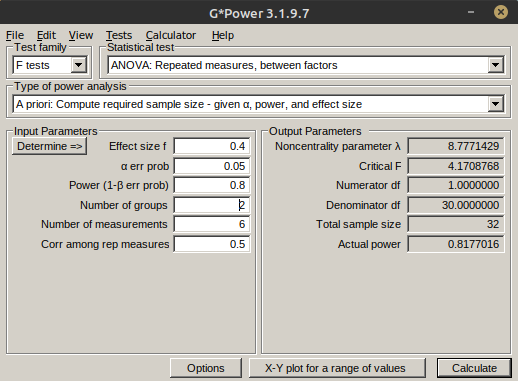
\includegraphics[width=\columnwidth]{Images/ANOVA_2.png}
    \caption{Screen capture from GPower software showing sample size calculation for an \textit{ANOVA: repeated measurements, between factors} test}
    \label{ANOVArepeatedbetween}
\end{figure}

\subsection{Ethical Considerations}\label{Ethics}
Due to the nature of this research, there are minimal ethical considerations that need to be taken into account. The participants will not be exposed to any potential risks outside of what they would experience under normal circumstances, although an effort has been made to keep the feedback form fairly condensed. This is to minimise any increased stress that the commitment of having to fill out the form may cause. Personal data will be collected, which will be stored and handled in compliance with GDPR regulations as discussed in the Data Management section. Care has also been taken to ensure no participant rights have been violated with respect to the Declaration of Helsinki\cite{goodyear2007declaration} or Nuremburg Code\cite{code1949nuremberg}\\
The artifact itself is of minimal risk, as it is collecting no personal information and does not have the potential to be weaponised. \\
Given these two factors, the project has been deemed medium risk and has such has been signed off by the research project Supervisor and Head of Subject, Dr Michael Scott, in accordance with Falmouth University's ethics policy\cite{falethicspolicy}.

\lstset{language = R}
\section{Data Analysis}
    Data for each hypothesis was analysed using repeated measures ANOVA \cite{carvadiaANOVA} using the R function \lstinline{aov} \cite{RaovDocs}. Three different ANOVA tests were then carried out, a one-way test against if the group was using the pipeline, a two-way test with the specific Team, and another two way test with the individual having an interaction effect upon their answer. An Akaike Information Criterion (AIC) \cite{AIC} test was then used to evaluate which of these models best fits our data, so we know which model to base our analysis off. \\
    Once determining the most accurate model, which for all hypothesise was the one-way ANOVA, the R function \lstinline{effectsize::omega_squared}\cite{RcohensfDocs} is used to calculate the effect size. Cohen's f was originally going to be used to compare effect sizes, however after consultation with more experienced academics $\eta^2$ was recommended instead. $\omega^2$ was then chosen as in the R documentation and elsewhere \cite{RcohensfDocs, statHowToOmegaSquared,ALBERS2018187}, it is recommended to use this over $\eta^2$ as it is less biased, especially for small sample sizes. As our sample size is only 25 results, this seems appropriate. The boundaries that will be used for contextualising the reported effect size are as follows\cite{field2013discovering}, where $x$ is the reported effect size:

    \begin{tabularx}{\linewidth}{r r c l}
        Very Small - & $0 > $ & $ x $ & $<=0.01$ \\
        Small - & $0.01 > $ & $ x $ & $<=0.06$ \\
        Medium - & $0.06 > $ & $ x $ & $<=0.14$ \\
        Large - & $0.14 > $ & $ x $ &  
    \end{tabularx}

    The $\omega^2$ value for many of these hypothesis was negative, and while this would normally be rounded to 0.00 this has been left as-is\cite{okada2017negative}.

    Data related to supervisor opinions was unable to be collected due to low uptake by teams \& even lower uptake by the supervisors for those teams. As only seven teams agreed to take part, and of these only two supervisors responded to the questionnaire, it was decided not to pursue these and leave them as avenues for future research.

    \subsection{The use of a CD pipeline will increase a supervisors confidence in their team's ability to deliver a new, working build each week, compared to team's not using a CD pipeline.}
        No Data Collected as discussed above.

    \subsection{The team's confidence and the supervisors confidence in being able to achieve everything within the scope of the project will be much more closely related with the use of a CD pipeline.}
        While supervisor data was not collected so a comparison can not be made, data regarding the team's confidence in their own scope was recorded. Pr($>$F) of 0.94, so ~94\% chance observed effect could be random, which is not statistically significant. The statistical power was -0.04.

    \subsection{A CD pipeline will help developers understand the current state of the project}
        Pr($>$F) of 0.68, so ~68\% chance observed effect could be random, which is not statistically significant. The statistical power was -0.04.

    \subsection{A CD pipeline will help developers to always know why the work they are doing is being done}
        Pr($>$F) of 0.707, so ~71\% chance observed effect could be random, which is not statistically significant. The statistical power was -0.04.

    \subsection{A team using a CD pipeline will refine their scope more often}
        Pr($>$F) of 0.0284 *, so ~3\% chance observed effect could be random, which is statistically significant. The size of this observed difference is also large, with an effect size of 0.16.

    \subsection{A team using a CD pipeline will do more playtesting}
        Pr($>$F) of 1, so 100\% chance observed change could be random. The statistical power was -0.04.

\section{Discussion of results}
    With an initial uptake of 7 teams and 34 people, and 27 responses to the questionnaires over four lots of data collection, the limited usefulness of the gathered results is no surprise. It is encouraging, however, to see some statistically significant results. Given the variation in the other results it is possible that further investigation with a larger sample size could still yield interesting results, as we are unable to rule out it does have an effect with our sample size.

\section{Issues and Limitations}
    limited sample size
    lack of responses from signed up attendees - no easy way of chasing people in person, email communication only so minimal accountability
    only one team had pipeline implemented, rest did not respond to invitation to set up pipeline with their team
    single experimental team mean's variation could be due just to random variation, extra samples would help to average that out

\section{Future Work}
    potential results but unaccounted for random variation means further work should be investigated
    recommend working with teams from the beginning of a year, and working with their academic supervisors to be able to chase team on responding to questionnaires and supporting them setting up and using the pipeline. Work with academics to identify suitable teams
    Worth considering the ethical considerations raised in Section \ref{Ethics} for future research. As this initial study points towards potential benefits consideration would have to be made to if this interference could disadvantage those not involved in the study. Making the study voluntary, being clearly transparent about potential advantages, would likely be enough to satisfy ethical concerns as all students are given equal opportunity to take part. 

\section{Conclusion}

CHECK OUT EDUCATION ROUNDTABLE AT GDC FOR SOFTWARE ENGINEERING, IF COULD LINK TO CONTEMPORARY ISSUES WITHIN EDUCATION WILL HELP WITH TIMELINESSs
\bibliographystyle{IEEEtran}
\bibliography{bibliography}

\section{Appendix}
\begin{figure}
    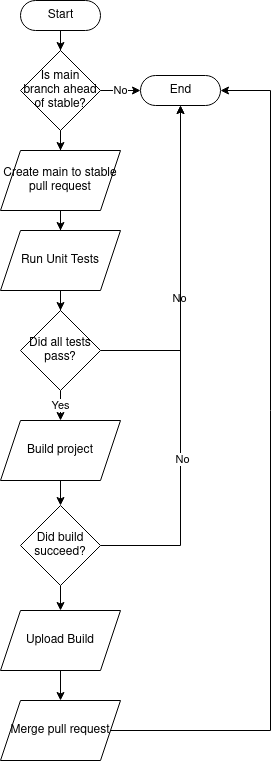
\includegraphics[width=0.95\columnwidth]{Images/CD.png}
    \caption{A diagram showing the flow of the Continuous Delivery system}
    \label{CDflow}
\end{figure}

\lstinputlisting[label=SCPullRequest, caption =Github Actions code to open a pull request from 'main' branch to 'stable/daily' branch at midnight each weeknight, captionpos=b]{Actions/.github/workflows/createPull.yml}

\lstinputlisting[label=SCBuildTest, caption=Github Actions code that runs on every opened Pull Request. Runs unit tests\, builds the project\, and then uploads it to steam, captionpos=b]{Actions/.github/workflows/BuildTestMain.yml}

\lstinputlisting[language=python, label=SCParse, caption=Python code that parses the results .csv generated by Microsoft Forms and exports only the useful data to a new .csv. User details are also encrypted., captionpos=b]{data_analysis/parsecsv.py}

\lstinputlisting[language =R, linerange=1-20, label=SCRAnalysis, caption =R code to perform ANOVA tests upon results after file is parsed with Python. Best fit analysis is then performed upon these tests., captionpos =b]{data_analysis/stat_analysis.r}

\end{document}